% ============================================================
%  HISTEROSALPINGOGRAFÍA (HSG)
%  Licenciatura en Imagenología --- UdelaR
%  Imagenología Especializada I, 2026
%  Lic. Camila Mier
%
%  IMPORTANTE: Este archivo NO tiene \documentclass ni
%  \begin{document}. Todo eso vive en main.tex.
%  Compila siempre desde main.tex con XeLaTeX.
% ============================================================

\chapter{Histeosalpingogrfia (HSG)}

% ============================================================
%  PUNTOS CLAVE PARA EL EXAMEN ORAL
% ============================================================
\begin{cajakeypoints}
\textbf{\color{azulprincipal} Puntos clave para el examen oral}
\begin{itemize}[noitemsep, topsep=2pt]
  \item La HSG es el \textbf{Gold Standard} para estudio de infertilidad: evalúa morfología uterina y \textbf{permeabilidad tubárica}.
  \item Se realiza en la \textbf{fase folicular}, entre el \textbf{7° y 12° día} del ciclo menstrual (endometrio delgado, riesgo de embarazo casi nulo).
  \item Requiere \textbf{BHCG negativa} antes del estudio.
  \item Catéter utilizado: \textbf{sholkoff 5--7 Fr}; el balón se infla a nivel del \textbf{istmo} con una jeringa de \textbf{10 mL de aire}.
  \item Volumen de contraste yodado hidrosoluble: aproximadamente \textbf{10 cc}.
  \item Contraindicaciones: infección genital activa, embarazo, lactancia.
  \item Útero bicorne: ángulo intercornual \textbf{$>$ 105°}. Útero septado: ángulo intercornual \textbf{$<$ 75°}.
  \item El paso bilateral de contraste a la cavidad peritoneal confirma la \textbf{permeabilidad tubárica bilateral}.
\end{itemize}
\end{cajakeypoints}

\vspace{1em}

% ============================================================
%  SECCIÓN 1 --- DEFINICIÓN
% ============================================================
\section*{Definición}

\begin{cajadefinicion}
La \textbf{histerosalpingografía (HSG)} es una prueba diagnóstica que consiste en la administración de contraste yodado a través del cuello cervical para evaluar la morfología de la cavidad uterina y el funcionalismo de las trompas de Falopio.
\end{cajadefinicion}

Durante muchos años ha sido la prueba de elección para el estudio de la morfología y funcionalismo de las trompas de Falopio. Con un correcto conocimiento anatómico y una buena calidad técnica permite también una adecuada evaluación de la \textbf{cavidad uterina} y el diagnóstico diferencial entre variantes de la normalidad y hallazgos patológicos.

\clearpage

% ============================================================
%  SECCIÓN 2 --- ANATOMÍA DE REFERENCIA
% ============================================================
\section*{Anatomía de Referencia}

Las estructuras que se opacifican durante la HSG son:

\begin{itemize}[noitemsep]
  \item \textbf{Cuello del útero} (cérvix): punto de entrada del catéter.
  \item \textbf{Cuerpo del útero}: cavidad principal evaluada.
  \item \textbf{Fundus del útero}: fondo uterino; su morfología orienta el diagnóstico de malformaciones.
  \item \textbf{Cuernos uterinos}: unión entre la cavidad y el origen de cada trompa.
  \item \textbf{Trompas de Falopio}: compuestas por istmo y ampolla; su permeabilidad es el objetivo principal del estudio.
  \item \textbf{Cavidad peritoneal}: la fuga bilateral de contraste confirma la permeabilidad tubárica completa.
\end{itemize}

% ============================================================
%  SECCIÓN 3 --- INDICACIONES Y DATOS CLÍNICOS
% ============================================================
\section*{Indicaciones y Datos Clínicos}

\subsection*{Indicaciones patológicas}

\begin{itemize}[noitemsep]
  \item \textbf{Estudio de la infertilidad} (malformación uterina y permeabilidad tubárica --- Gold Standard).
  \item Abortos de repetición.
  \item Malformaciones congénitas uterinas.
  \item Valoración \textbf{pre y post-quirúrgica}, especialmente de la ligadura de trompas.
  \item Hemorragia uterina anormal.
  \item Poscesárea.
  \item Embarazo tubárico (luego de salpingotomía).
  \item Post-miomectomía (adherencias intrauterinas).
\end{itemize}

% ============================================================
%  SECCIÓN 4 --- PREPARACIÓN Y CONTRAINDICACIONES
% ============================================================
\section*{Preparación Previa y Contraindicaciones}

\subsection*{Verificaciones previas obligatorias}

\begin{enumerate}[noitemsep]
  \item Verificar que la paciente \textbf{no esté embarazada} (BHCG negativa).
  \item Interrogar sobre \textbf{antecedentes de infecciones genitales}.
  \item Evaluar \textbf{reacción alérgica} al medio de contraste yodado; algunos pacientes requieren preparación previa.
  \item Confirmar que el estudio se realiza en la \textbf{fase folicular} (entre el 7° y el 12° día del ciclo menstrual).
  \item Obtener \textbf{consentimiento informado} firmado.
\end{enumerate}

El procedimiento se realiza de modo \textbf{ambulatorio} y es muy rápido.

\clearpage

\subsection*{Contraindicaciones}

\begin{cajariesgo}
\textbf{Contraindicaciones absolutas:}
\begin{itemize}[noitemsep, topsep=2pt]
  \item Infección genital activa.
  \item Embarazo (BHCG positiva).
  \item Lactancia.
\end{itemize}
\end{cajariesgo}

\clearpage
% ============================================================
%  SECCIÓN 5 --- PROTOCOLO DE PROCEDIMIENTO
% ============================================================
\section*{Protocolo de Procedimiento}

\subsection*{Posición de la paciente}

La paciente se acuesta sobre la mesa de radiología digital en \textbf{decúbito supino en posición ginecológica}.

\subsection*{Pasos del procedimiento}

\begin{enumerate}[noitemsep]
  \item Desinfección del \textbf{periné y genitales externos}.
  \item Introducción del \textbf{espéculo}, eventualmente lubricado con vaselina.
  \item Desinfección del \textbf{cuello del útero} con solución antiséptica aplicada con pinzas y compresas.
  \item Introducción del \textbf{catéter sholkoff 5--7 Fr} a través del orificio externo del cuello, avanzando hasta el \textbf{istmo}, donde se infla el balón con una \textbf{jeringa de 10 mL rellena de aire}.
  \item Inyección lenta de \textbf{contraste yodado hidrosoluble}, volumen aproximado de \textbf{10 cc}.
\end{enumerate}

% ============================================================
%  SECCIÓN 6 --- PROYECCIONES RADIOLÓGICAS
% ============================================================
\section*{Proyecciones Radiológicas}

Las proyecciones se realizan en el siguiente orden secuencial:

{\renewcommand{\arraystretch}{1.35}
\begin{center}
\begin{tabular}{>{\bfseries}p{1.2cm} p{4.5cm} p{7.5cm}}
\hline
N° & Proyección & Lo que se evalúa \\
\hline
Previa & RX de pelvis sin contraste & Calcificaciones pélvicas basales. \\[0.5em]
\hline
1 & AP pelvis --- relleno precoz de la cavidad & Defectos o anomalías del contorno uterino; más fácil de detectar con poca cantidad de contraste. \\[0.5em]
\hline
2 & AP pelvis --- cavidad distendida & Forma de la cavidad; pequeñas irregularidades de los contornos que pueden enmascararse con el medio de contraste. \\[0.5em]
\hline
3 & Oblicuas bilaterales & Despejar y visualizar individualmente cada trompa de Falopio. \\[0.5em]
\hline
4 & AP pelvis --- paso peritoneal bilateral & Confirmación de permeabilidad tubárica bilateral: paso de contraste a peritoneo de forma bilateral. \\[0.5em]
\hline
5 & Post-evacuación & Comprobar la \textbf{libre distribución} del contraste en la cavidad peritoneal; ausencia de colecciones localizadas. \\
\hline
\end{tabular}
\end{center}
}

\clearpage
\begin{figure}
    \centering
    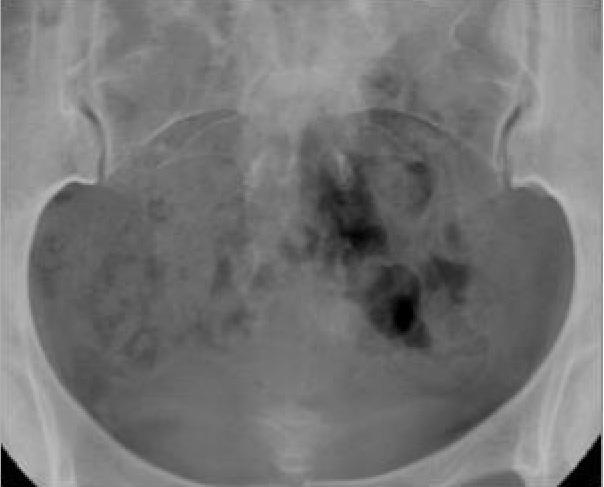
\includegraphics[width=0.5\linewidth]{imagenes/hist1.png}
    \caption{Rx 0 - de pelvis sin contraste}
    \label{fig:h1}
\end{figure}

\begin{figure}
    \centering
    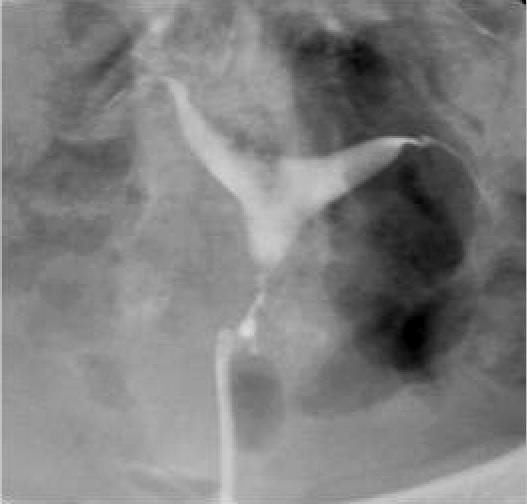
\includegraphics[width=0.5\linewidth]{imagenes/hist2.png}
    \caption{Rx 1 - Llenado precoz}
    \label{fig:h2}
\end{figure}

\begin{figure}
    \centering
    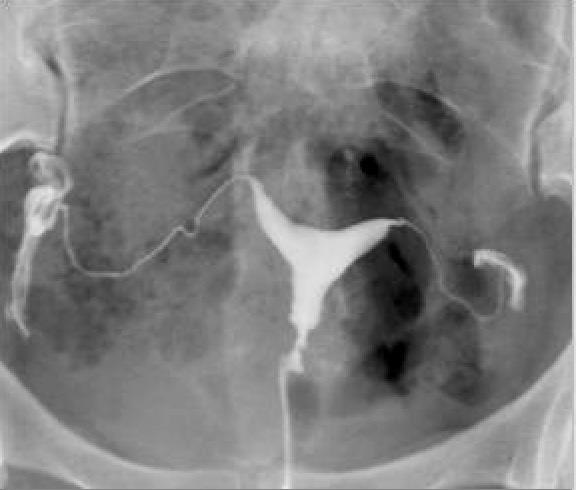
\includegraphics[width=0.5\linewidth]{imagenes/hist3.png}
    \caption{Rx 2 - Cavidad distendida}
    \label{fig:h3}
\end{figure}

\begin{figure}
    \centering
    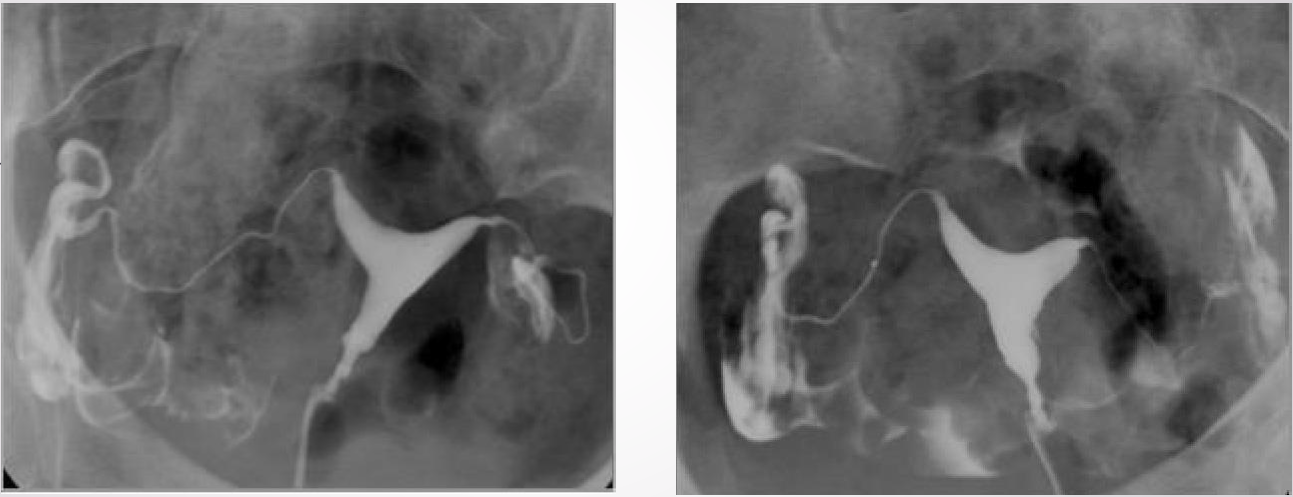
\includegraphics[width=1\linewidth]{imagenes/hist4.png}
    \caption{Rx 3 - Oblicuas}
    \label{fig:h4}
\end{figure}

\begin{figure}
    \centering
    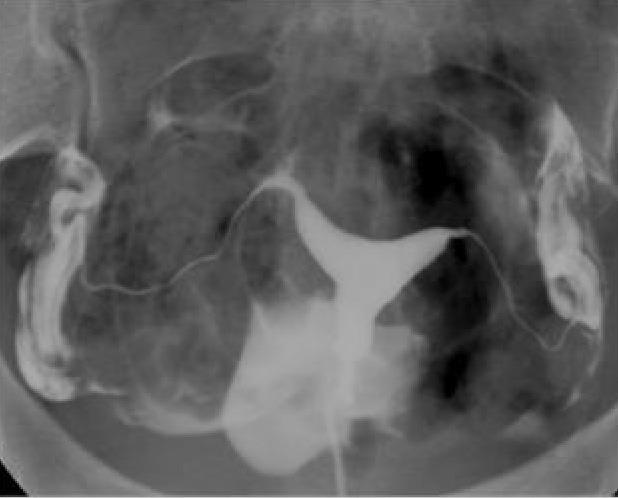
\includegraphics[width=0.5\linewidth]{imagenes/hist5.png}
    \caption{Rx 4 - Paso de MC al peritoneo}
    \label{fig:h5}
\end{figure}

\begin{figure}
    \centering
    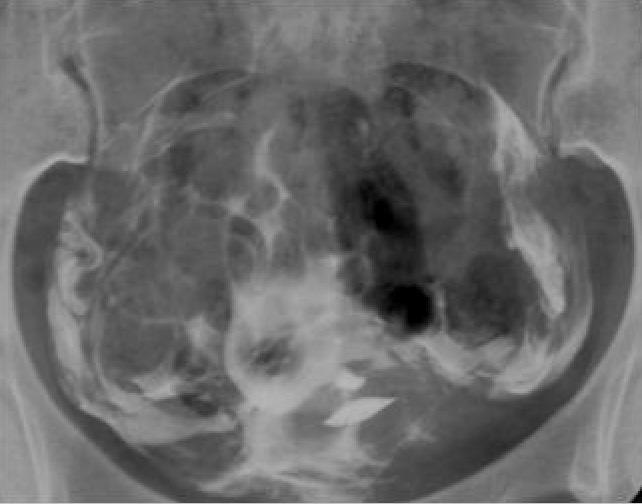
\includegraphics[width=0.5\linewidth]{imagenes/hist6.png}
    \caption{Rx 5 - Post evacuación}
    \label{fig:h6}
\end{figure}

\clearpage

% ============================================================
%  SECCIÓN 7 --- HALLAZGOS PATOLÓGICOS
% ============================================================
\section*{Hallazgos Patológicos Principales}

\subsection*{Espasmo tubárico}

Obstrucción tubárica uni o bilateral que puede afectar a cualquier segmento de la trompa. La etiología más frecuente es la \textbf{infecciosa}. En la HSG se evidencia como ausencia de paso de contraste más allá del sitio de obstrucción.

\begin{figure}[h]
    \centering
    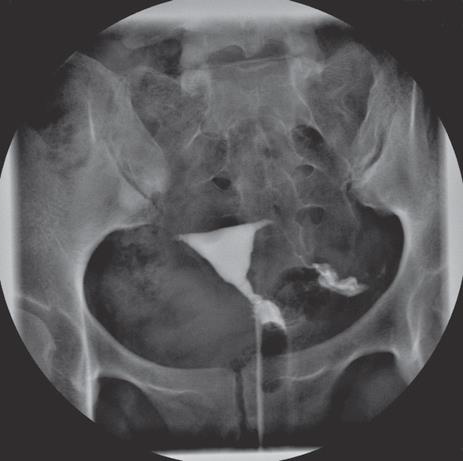
\includegraphics[width=0.5\linewidth]{imagenes/espasmo tubarico.png}
    \caption{Espasmo tubarico}
    \label{fig:h7}
\end{figure}

\subsection*{Malformaciones congénitas uterinas}

Todas derivan de anomalías en el desarrollo o fusión de los \textbf{conductos de Müller (paramesonéfricos)}.

\begin{center}
\begin{tabular}{>{\bfseries}p{2.8cm} p{5.5cm} p{5cm}}
\hline
Malformación & Mecanismo & Aspecto en HSG \\
\hline
Útero unicorne & Ausencia de desarrollo de un conducto de Müller. & Una sola cavidad con una trompa; cavidad y trompa desviadas lateralmente. \\[0.5em]
\hline
Útero didelfo & Falta de fusión completa de los conductos mullerianos. & Dos cavidades uterinas independientes con dos cuellos; requiere cateterización de \textbf{ambos} orificios cervicales. \\[0.5em]
\hline
Útero bicorne & Fusión incompleta de los conductos paramesonéfricos. & Cérvix único con dos cuernos uterinos \textbf{divergentes}; ángulo intercornual \textbf{$>$ 105°}. \\[0.5em]
\hline
Útero septado & Reabsorción incompleta del septo uterovaginal. & Dos cavidades separadas por un septo; ángulo intercornual \textbf{$<$ 75°}. \\
\hline
\end{tabular}
\end{center}

\begin{figure}
    \centering
    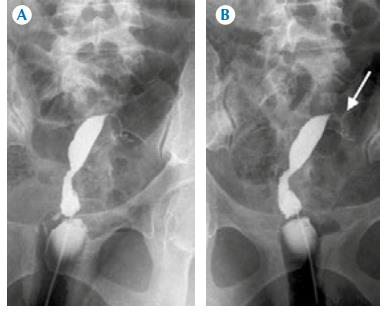
\includegraphics[width=0.5\linewidth]{imagenes/unicorne.png}
    \caption{Útero unicorne}
    \label{fig:h8}
\end{figure}

\begin{figure}
    \centering
    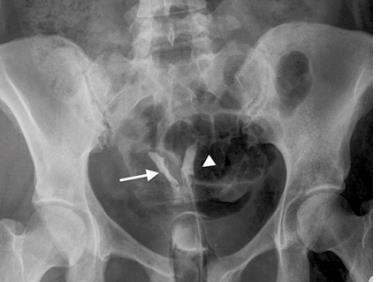
\includegraphics[width=0.5\linewidth]{imagenes/didelfo.png}
    \caption{Útero didelfo}
    \label{fig:h9}
\end{figure}

\begin{figure}
    \centering
    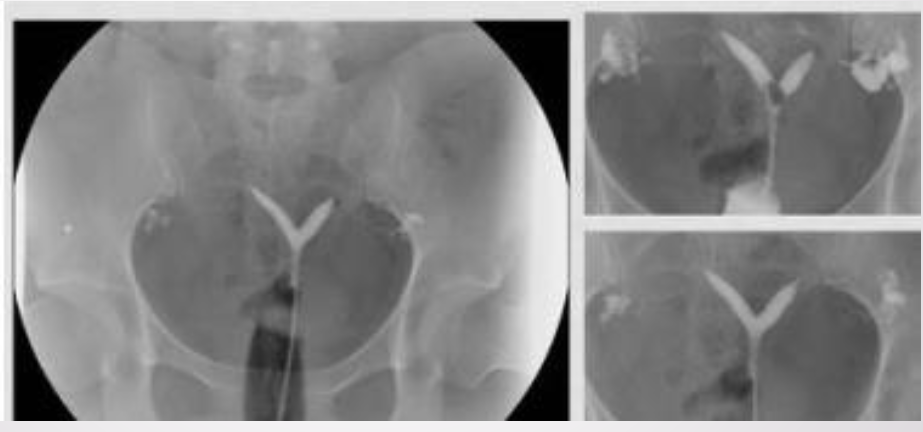
\includegraphics[width=0.5\linewidth]{imagenes/bicorne.png}
    \caption{Útero bicorne}
    \label{fig:h10}
\end{figure}

\begin{figure}
    \centering
    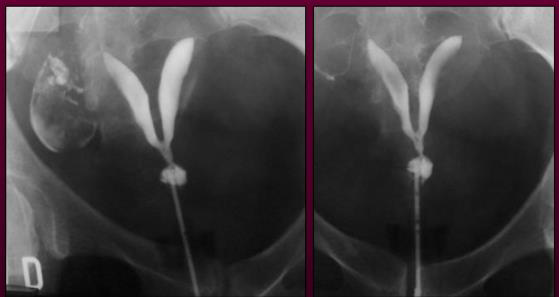
\includegraphics[width=1\linewidth]{imagenes/septado.png}
    \caption{Útero septado}
    \label{fig:h11}
\end{figure}

\clearpage

\begin{cajakeypoints}
\textbf{Diagnóstico diferencial clave:} Bicorne vs. septado se distingue por el \textbf{ángulo intercornual}: $>105°$ = bicorne; $<75°$ = septado.
\end{cajakeypoints}

% ============================================================
%  CIERRE --- ESQUEMA MENTAL FINAL
% ============================================================
\section*{Esquema Mental --- Repaso Final}

\begin{cajakeypoints}
\begin{center}
\textbf{\color{azulprincipal}
  BHCG negativa $\rightarrow$ Fase folicular (día 7--12) $\rightarrow$ Sholkoff 5--7 Fr (istmo) $\rightarrow$ 10 cc contraste $\rightarrow$ Serie de 5 proyecciones}\\[0.4em]
\textbf{\color{naranjadestacado}
  Gold Standard de infertilidad. Permeabilidad confirmada: paso bilateral de contraste a peritoneo.}\\[0.3em]
Balón: jeringa 10 mL de aire \quad Bicorne: $>105°$ \quad Septado: $<75°$ \quad Didelfo: cateterizar ambos cuellos\\[0.3em]
\textbf{Protocolo:} simple $\to$ relleno precoz $\to$ cavidad distendida $\to$ oblicuas $\to$ paso peritoneal $\to$ post-evacuación
\end{center}
\end{cajakeypoints}

\vspace{1em}
\hrule
\vspace{0.5em}
